We have previously defined \textit{TinyFace} as a face detector application, powered by neural networks, and running in a TensorFlow-Lite interpreter environment, where certain steps have been undertaken to reduce model size and complexity. This chapter will present a working application where this has been made possible. \par
As previously discussed, there are esentially 4 steps to building \textit{TinyFace}: gathering data, experimenting with convolutional neural-network model architectures, training, and, finally, evaluating inference performance. With it being an iterative process, this means that after running through all 4 steps, we must go back to step 1 and try improving our model's performance even more. \par
\section{Webscrapper}
Webscrapper is a Selenium-based automatic web-scraping tool, which can search for, download, pre-process, crop and add padding to, sort, filter and save images where faces are present. We need Webscapper to build datasets for training.
\section{Compressed Squeezenet}
\subsection{Goals}
\subsection{Architecture}
See \textit{Figure \ref{netron_sqnet}} for a fully expanded description.

\begin{figure}[!tbp]
\centering
\subfloat[Top Third]{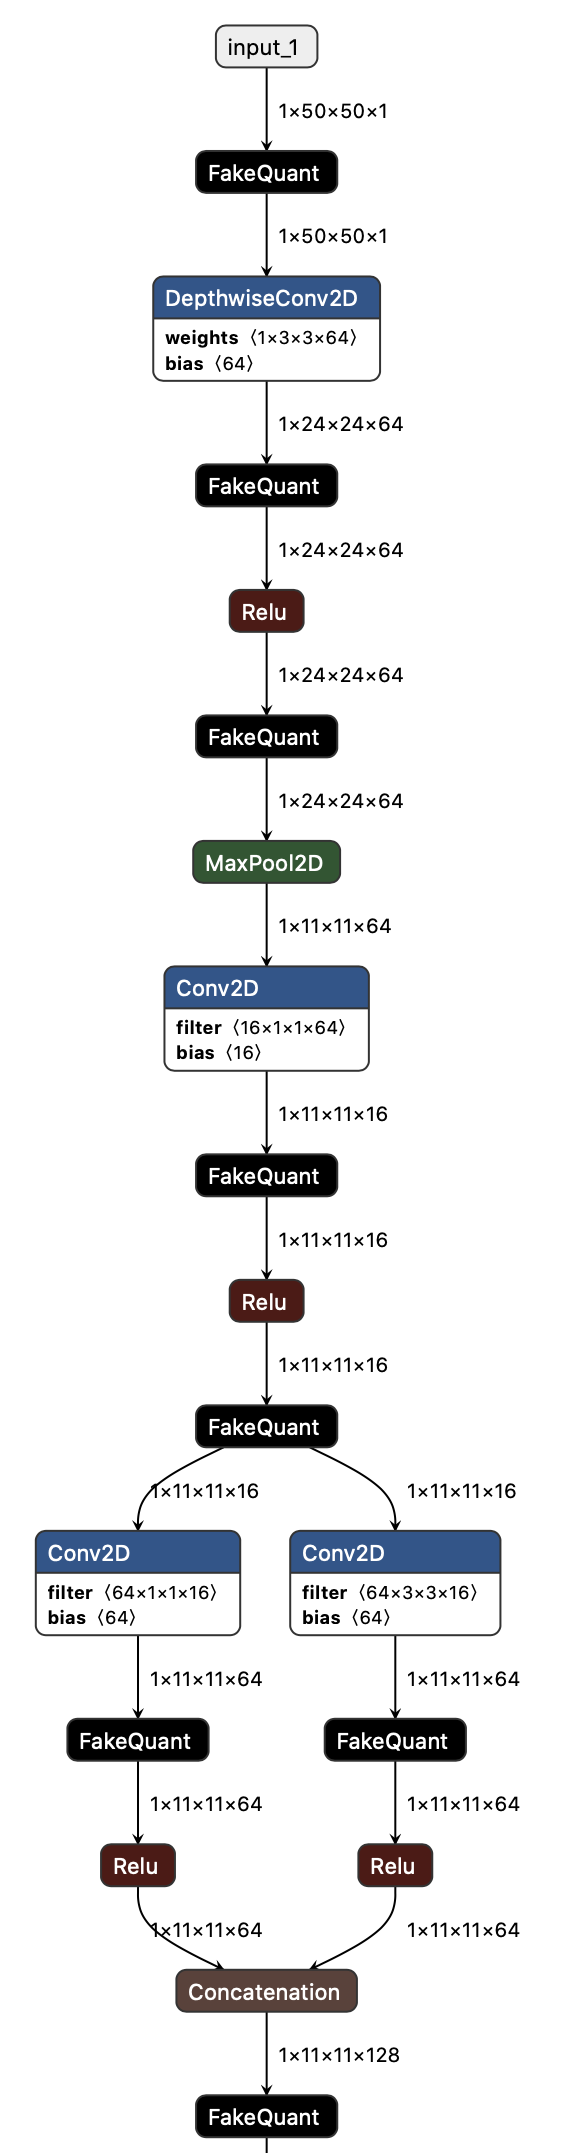
\includegraphics[height = 20 cm]{images/netron_sqnet_1.png}
\label{fig:f1}}
\hfill
\subfloat[Middle Third]{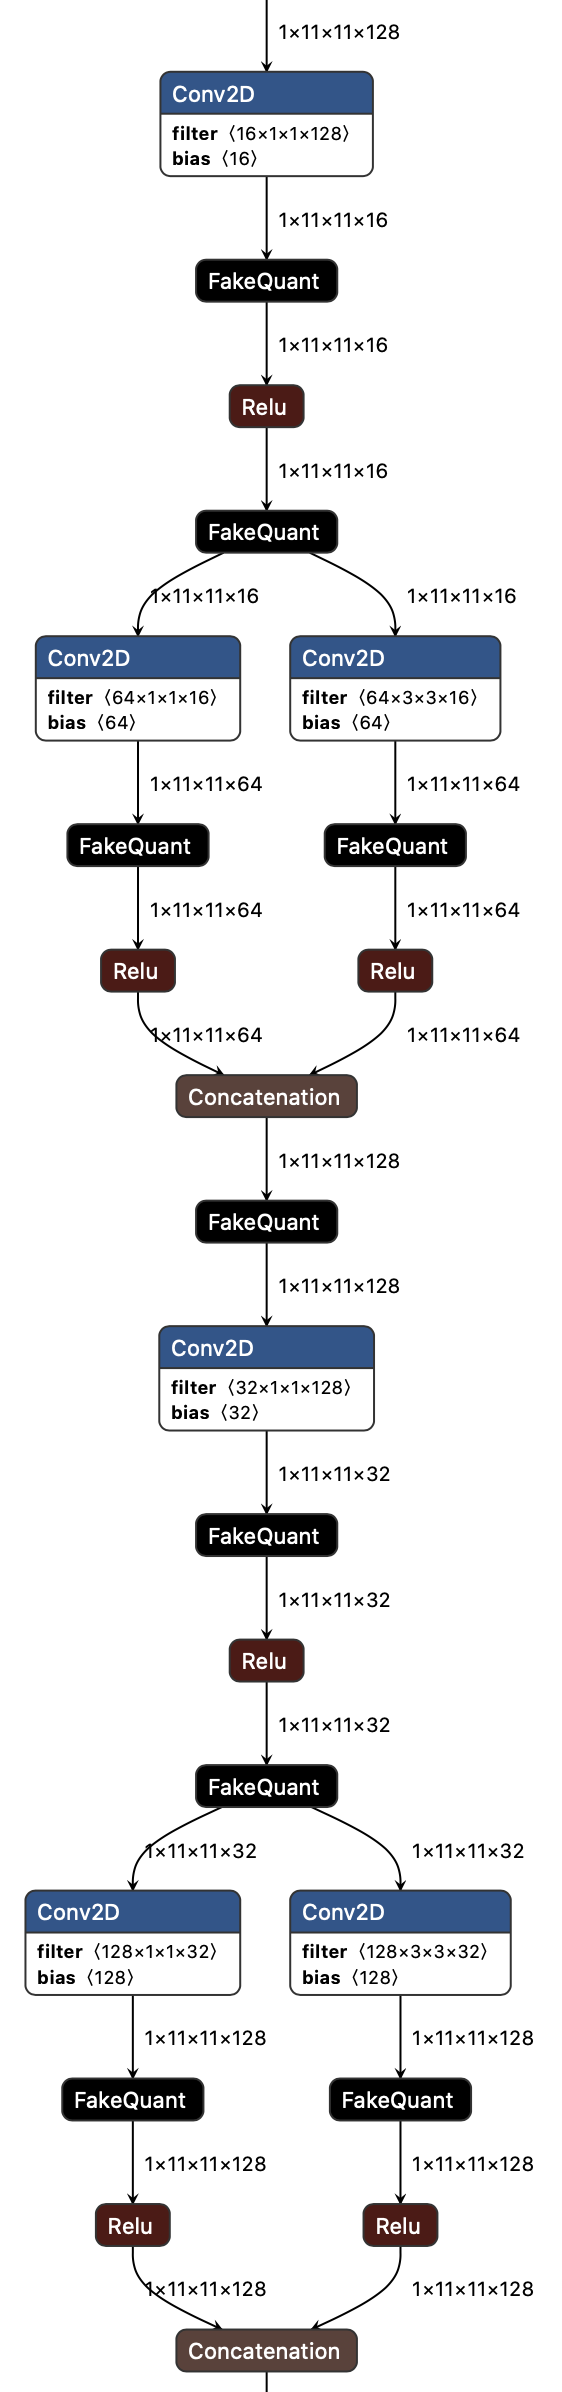
\includegraphics[height = 20 cm]{images/netron_sqnet_2.png}
\label{fig:f2}}
\subfloat[Bottom Third]{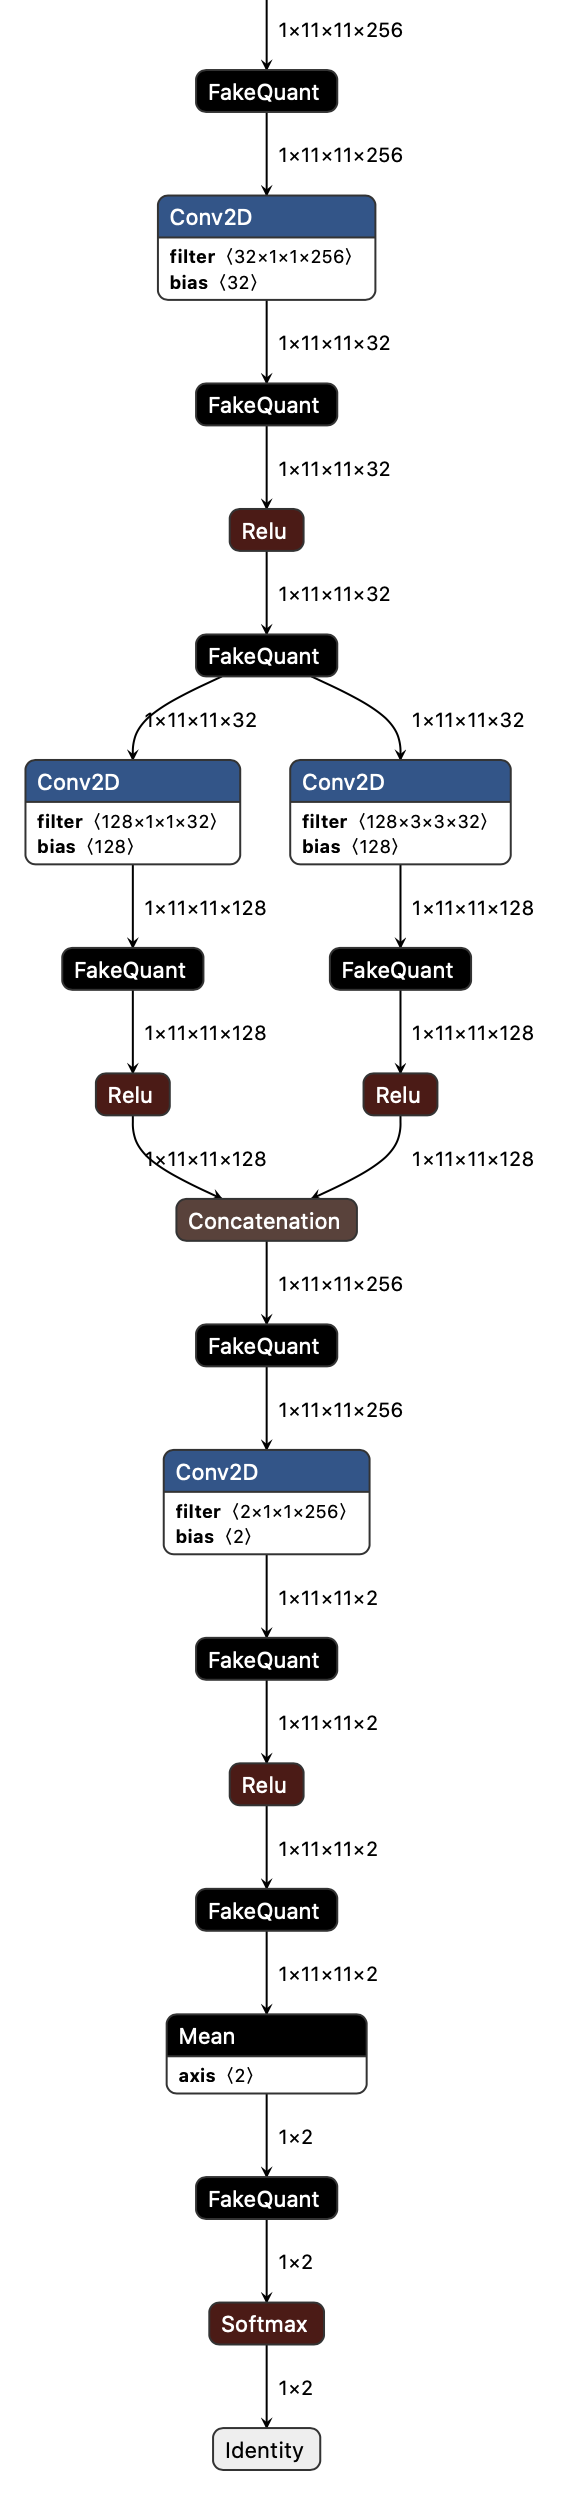
\includegraphics[height = 20 cm]{images/netron_sqnet_3.png}
\label{fig:f3}}
\caption{Fully expanded vizualization of trained Squeezenet. Note that the image was divided so it would fit on one page. Generated from TF-Lite file by Netron. \cite{netron}}
\label{netron_sqnet}
\end{figure}


\section{The Model Trainer}
\subsection{Goals}
\subsection{Architecture}
\subsection{Datasets}
\section{The Webcam App}
\subsection{Code Structure}
\subsection{Inference Performance}
